%!TEX root = ../main.tex
\chapter{Schätzer}
\section{Allgemeines zum Schätzen}
Beim Schätzen wollen wir von einer Beobachtung einer (teilweise) unbekannten Verteilung auf Parameter der Verteilung schließen.

Das kann bedeuten, dass man versucht aus einer Stichprobe zu folgern, ob es sich zum Beispiel um eine Normalverteilung handelt.
Aber ebenso kann man zum Beispiel den Parameter $\mu$ der Normalverteilung schätzen.

Man sieht sofort dass man beim Schätzen einige Angaben entweder wissen oder Annahmen treffen muss.
Selbstverständlich kann man nur Parameter einer Verteilung schätzen wenn man annimmt dass es sich um diese Verteilung handelt.

Es gibt verschiede Arten zu Schätzen, so kann man beispielsweise einen Bereich angeben in dem sich der Parameter mit einer gewissen Sicherheit befindet (Lage- oder Intervallschätzer).




\section{Intervallschätzer}
Die Intervallschätzer geben ein Intervall an, in dem sich der zu schätzende Parameter höchstwahrscheinlich befindet. Hierbei sind möglichst kleine Intervalle bei einer hohen Sicherheit natürlich gewünscht, aber diese Einschränkungen widersprechen sich. 
Verkleinert man das Intervall wird die Sicherheit, dass der geschätze Parameter wirklich enthalten ist im Allgemeinen kleiner.


\subsection{Mit Tschebyscheff-Ungleichung}

\subsection{Über die Verteilungsfunktion}





\section{Maximum-Likelihood-Schätzer}
Die Maximum-Likelihood-Schätzmethode verwendet eine sogenannte Likelihoodfunktion $L$. Diese ist abhängig vom zu schätzenden Parameter $\alpha$, man sucht dann den Wert für $\alpha$ so, dass $L(\alpha)$ ein Maximum annimmt. Häufig wird dieser Wert mit einem Dach gekennzeichnet. 

Das Ergebnis dieses Schätzers wäre also allgemein
\begin{equation*}
	\hat\alpha = \underset\alpha\argmax L(\alpha)
\end{equation*}

Hierbei hängt die Likelihoodfunktion davon ab, was bei welcher Verteilung geschätzt wird. 


Wir wollen den Maximum-Likelihood-Schätzer anhand der Binomialverteilung betrachten.
Hierbei macht nur Schätzen des Parameters $p$ Sinn, denn selbst wenn nur eine einzige Stichprobe vorliegt, sieht man sofort welchen Wert $n$ hat.

Es liegt also eine Verteilung 
\begin{equation*}
	X\sim\binomial(n,p)
\end{equation*}
zugrunde, hierbei ist $n$ bekannt und fest, $p\in(0,1)$ wollen wir herausfinden.

Liegt uns nun eine Stichprobe $\omega$ vor, so ist auch $X(\omega)=k$ bekannt als die Anzahl Treffer in den $n$ Bernoulli-Experimenten.

Zum Schätzen fehlt uns noch die Likelihoodfunktion, diese ist hier
\begin{equation*}
	L:(0,1)\rightarrow[0,1], \enspace L(p)=P_p(X=k)=\binom{n}{k}*p^k(1-p)^{n-k}
\end{equation*}

Das heißt, es ist die Wahrscheinlichkeit dass $X$ mit Trefferwahrscheinlichkeit $p$ (als Parameter!) den Wert $k$ annimmt. Man sieht, dass diese Funktion ihr Maximum bei dem Wert für $p$ annimmt, unter dem es am wahrscheinlichsten ist, die Stichprobe $\omega$ zu erhalten.
\begin{center}
	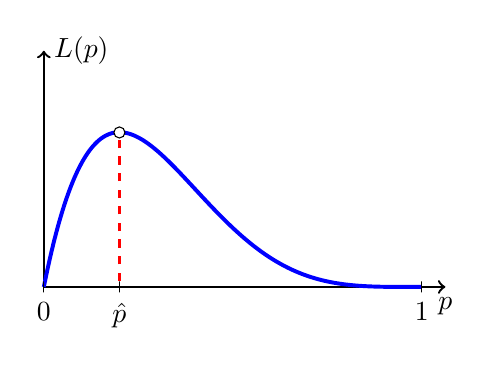
\begin{tikzpicture}[scale=0.6]
		\draw[->, line width=0.3mm] (0,0) to (8.5,0) node[below] {$p$};
		\draw[->, line width=0.3mm] (0,0) to (0,5) node[right] {$L(p)$};

		\draw[line width=0.5mm,scale=8,domain=0:1,smooth,variable=\x,blue, samples=100] plot ({\x},{5*\x * ((1-\x)^(4))});


		%\draw[line width=0.5mm,scale=8,domain=0.001:1,smooth,variable=\x,green, samples=100] plot ({\x},{0.15*(5*(1-\x)^4-20*\x*(1-\x)^3)});	

		\draw (1.6,0) node (hatp) [rectangle,inner sep = 0pt,minimum size = 0pt,minimum height=4pt,draw, label={below:$\hat p$}] {};
		\draw (1.6,3.27) node (Lhatp) [fill = white,circle,inner sep = 0pt,minimum size = 4pt,draw] {};

		
		\draw (0,0) node (null) [rectangle,inner sep = 0pt,minimum size = 0pt,minimum height=4pt,draw, label={below:$0$}] {};
		\draw (8,0) node (eins) [rectangle,inner sep = 0pt,minimum size = 0pt,minimum height=4pt,draw, label={below:$1$}] {};
		

		\draw[red, line width=0.3mm, dashed] (hatp) -- (Lhatp);
			
	\end{tikzpicture}	
\end{center}
Den Wert $\hat p$ zu berechnen würde hier durch Ableiten und anschließendem Bestimmen der Nullstelle erfolgen
\begin{equation*}
	\frac{\diff}{\diff p}L(\hat p)\overset!= 0.
\end{equation*}

\paragraph{Beispiel:}
Wir wollen dies nun nochmal an einem Beispiel veranschaulichen. Wir schätzen wiederum $p$ einer Binomialverteilung, schließen damit später aber auf einen anderen Wert.
\begin{eBox}{}{}
	Um die Populationsgröße $N$ einer Fischart in einem See zu schätzen, gehen wir folgendermaßen vor: Wir markieren von dieser Art $m=50$ Fische in einem See, fangen später $n=200$ Stück und stellen fest, dass $k=16$ davon markiert sind.

	Wir nehmen an, dass das Untersuchen der Stichprobe auf Markierungen eine Folge von $n$ unabhängigen Bernoulli-Experimenten mit Trefferwahrscheinlichkeit $p=\frac mN$ ist. Also beschreibt $p$ den Anteil der markierten Fische im See.
\end{eBox}
Wir verwenden die zuvor besprochene Likelihoodfunktion $L(p)$, denn mit $p=\frac mN$ können wir auf $N$ schließen. 

Sei $X$ eine Zufallsvariable die die Anzahl markierter Fische in der Stichprobe beschreibt, damit ist $X \sim \binomial(200,p)$ verteilt. 

Die Likelihoodfunktion ist mit diesen Werten
\begin{equation*}
	L(p)=P_p(X=k)=\binom{200}{k}* p^{k}(1-p)^{200-k}
\end{equation*}
Damit folgt
\begin{align*}
	\frac{\diff}{\diff p}L(p) &= \binom{200}{k}*\left[ k*p^{k-1}(1-p)^{200-k} - p^k*(200-k)*(1-p)^{200-k-1}\right]\\
	&=\underbrace{\binom{200}{16}* p^{k-1}(1-p)^{200-k-1}}_{>0} * \left[ k(1-p)-200p+kp \right]\\
\end{align*}
Da wir uns für Nullstellen interessieren, betrachten wir nur noch den rechten Teil und erhalten
\begin{align*}
	k(1-\hat p)-200\hat p+k\hat p&\overset != 0\\
	k-k\hat p-200\hat p+k\hat p &= 0\\
	k-200\hat p&=0
\end{align*}
Für unsere Stichprobe $\omega$ ist $X(\omega)=k=16$, damit ist
\begin{align*}
	\hat p =\frac{m}{N} =\frac k{200}\Rightarrow N&=\frac {m*200}{k}\\
	\Rightarrow N &= \frac{50*200}{16} = 625
\end{align*}

Wir haben damit die Populationsgröße der Fischart auf 625 geschätzt.





\section{Kleinste Quadrate-Schätzer}



\section{Bayes-Schätzer}



Wir betrachten die Zufallsvariable $X$ mit dem zugehörigen Wahrscheinlichkeitsraum $(X(\Omega), P_\theta)$. Hierbei wollen wir den Parameter $\theta$ schätzen. 

Der Bayes-Schätzer stellt eine komplett andere Herangehensweise an das Schätzen dar, hier wird der gesuchte Parameter als eine Zufallsvariable aufgefasst. So können weitere Annahmen wie Erfahrung aus anderen Experimenten oder ein grobes Vorwissen über den Sachverhalt in den Schätzvorgang eingehen.

Achtung, die Werte der Zufallsvariable $\theta$ werden ebenfalls $\theta$ genannt.
\begin{enumerate}
	\item 
	Wir betrachten also zunächst die gemeinsame Dichte $f(x,\theta)$ wobei $x\in X(\Omega)$ und $\theta\in \Theta\subseteq[0,1]$. 

	Der einfachere Fall ist hierbei, wenn es sich sowohl bei $X$ als auch $\theta$ um diskrete Zufallsvariablen handelt (wir betrachten nur diesen), dann kann man die gemeinsame Verteilung durch die Kontingenztafel darstellen
	$$
	\begin{array}{|c|cccc|c|}
		\hline \text{gem. Dichte}&x_1&x_2&x_i&x_m&\\\hline
		\theta_1&f(x_1,\theta_1)&f(x_2,\theta_1)&\cdots&f(x_m,\theta_1)&\\
		\theta_2&f(x_1,\theta_2)&\ddots&&&\\
		\vdots&\vdots&&f(x_i,\theta_j)&\vdots&f(\theta_j)=\sum_{i=1}^m f(x_i,\theta_j)\\
		\theta_n&f(x_1,\theta_n)&\cdots&&f(x_m,\theta_n)&\\\hline
		\text{Randdichte}&&&f(x_j)=\sum_{j=1}^n f(x_i,\theta_j)&&\\\hline
	\end{array}
	$$

	\item Nun kann man die bedingte Verteilung von $X$ unter gegebenem $\theta$ darstellen als
	\begin{equation*}
		f(x_i|\theta_j)=P_\theta(X=x_i)
	\end{equation*}
	Da hierbei $\theta$ nun fest gewählt ist, kann man dies problemlos berechnen.

	\item Jetzt kommt der Punkt an dem die Besonderheit der Bayes-Schätzung eingeht, man legt eine sogenannte \emph{a-priori-Dichte} für $\theta$ fest. 
	Zum Beispiel kann dies eine Gleichverteilung auf ganz $\Theta$ sein, das würde bedeuten, man hat kein besonderes Vorwissen über $\theta$.
	Man kann aber genaso vorgeben, dass einige Werte für $\theta$ wahrscheinlicher als andere sind, dies beeinflusst das Ergebnis und kann so zu genaueren Schätzergebnissen führen.

	\item Als letztes berechnet man noch die Randdichte von $X$, unabhängig vom Parameter $\theta$
	\begin{align*}
		f(x_j)&=P(X=x_j)=\sum_{i=1}^n f(x_j|\theta_i)*f(\theta_i)\quad\text{(Satz v. d. totalen Wahrscheinlichkeit)}\\
		&=\sum_{i=1}^n f(x_j,\theta_i)
	\end{align*}
\end{enumerate}

Jetzt führen wir ein Experiment durch. Liegt uns nun eine Stichprobe $\tilde x\in\simpleset{x_1,\ldots,x_m}$ vor, so können wir damit von der a-priori-Dichte auf die sogenannte a-posteriori-Dichte $f(\theta_i,\tilde x)$ schließen.
Wir erhalten also eine Aussage über die Wahrscheinlichkeit eines $\theta_i$ bei gegebenem Ergebnis $\tilde x$.
\begin{align*}
	f(\theta_i|\tilde x)&=\frac{f(\tilde x|\theta_i)*f(\theta_i)}{f(\tilde x)}\quad\text{(Satz von Bayes)}\\
	&=\frac{f(\tilde x,\theta_i)}{\sum_{k=1}^m f(\tilde x|\theta_k) * f(\theta_k)}
\end{align*}
